% \subsection{Giới thiệu đề tài}
% \subsubsection{Tổng quan về ngành công nghiệp nhà hàng}
% Tính đến năm 2023, ngành dịch vụ thực phẩm (bao gồm khách sạn, nhà hàng và dịch vụ thể chế) đã đạt tổng giá trị 26,9 tỷ USD, với mức tăng trưởng 14,7\%. Mặc dù phải đối mặt với nhiều thách thức như lạm phát, chi phí vận hành tăng cao và sự cạnh tranh khốc liệt, ngành này đã phục hồi mạnh mẽ và gần như đạt doanh thu tương đương với thời kỳ trước đại dịch. Trong nửa đầu năm 2024, doanh thu từ dịch vụ lưu trú, thực phẩm và đồ uống đạt 24,1 tỷ USD, tăng 12,5\% so với cùng kỳ năm trước \cite{USDA}. 
% \\
% % cái ở trên ref từ https://apps.fas.usda.gov/newgainapi/api/Report/DownloadReportByFileName?fileName=Food%20Service%20-%20Hotel%20Restaurant%20Institutional%20Annual_Ho%20Chi%20Minh%20City_Vietnam_VM2024-0038.pdf

% \begin{figure}[H]
%     \centering
%     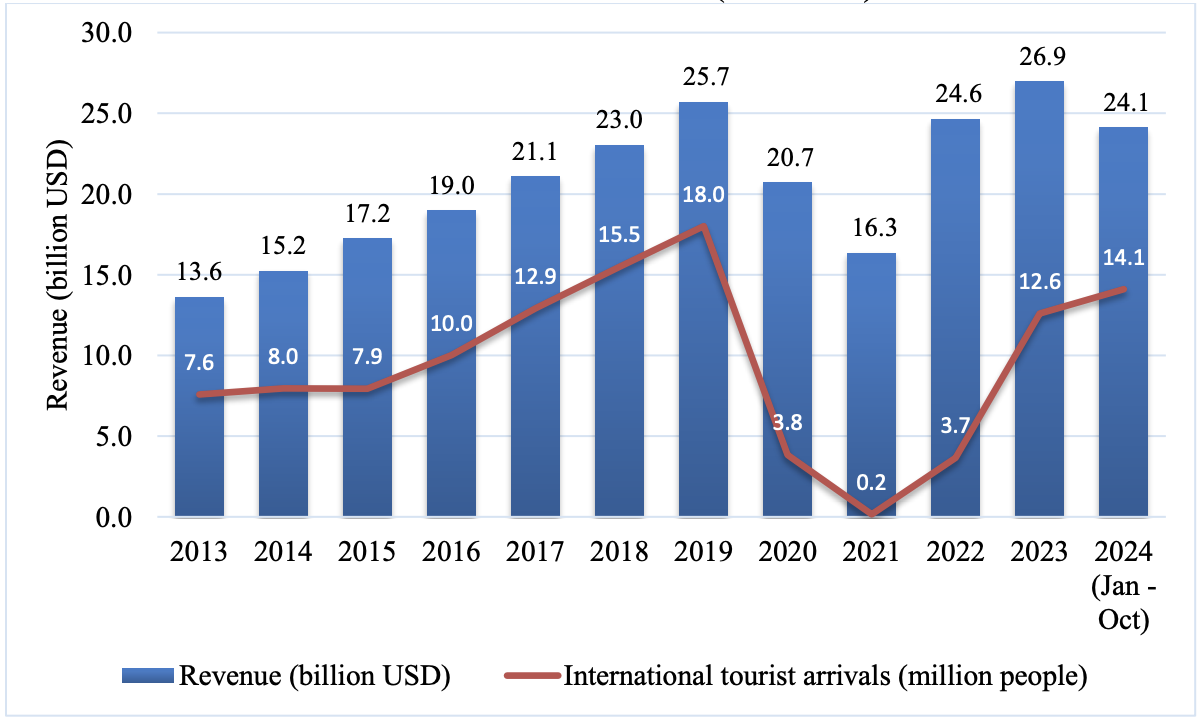
\includegraphics[width=15cm]{Images/resindus.png}
%     \caption{Doanh thu từ Dịch vụ Lưu trú, Ăn uống và Số lượng Du khách Quốc tế từ năm 2013 đến năm 2024. Nguồn: Post calculations; Vietnam’s General Statistics Office.}
%     \label{fig:enter-label}
% \end{figure}

% Trong bối cảnh công nghệ số ngày càng phát triển mạnh mẽ, việc áp dụng các giải pháp công nghệ vào quản lý và vận hành doanh nghiệp không chỉ là xu hướng mà còn là yếu tố quan trọng giúp nâng cao hiệu quả hoạt động và cải thiện trải nghiệm khách hàng. Đặc biệt, đối với ngành dịch vụ ăn uống, đặc biệt là các nhà hàng, việc quản lý quy trình đặt món và phục vụ khách hàng có thể gặp nhiều khó khăn và thách thức do tính chất phức tạp của công việc, cũng như yêu cầu phải đáp ứng nhu cầu đa dạng của khách hàng. \\

% Phương pháp quản lý truyền thống, dựa chủ yếu vào ghi chép thủ công và giao tiếp trực tiếp, đã bộc lộ nhiều hạn chế, chẳng hạn như dễ mắc sai sót, khó theo dõi lịch sử đặt món và tốn thời gian trong quá trình vận hành. Những vấn đề này không chỉ làm giảm hiệu quả công việc mà còn ảnh hưởng xấu đến trải nghiệm của khách hàng, đặc biệt là trong môi trường cạnh tranh ngày càng gay gắt trong ngành. \\

% Dự án này được triển khai nhằm giải quyết những vấn đề đó thông qua việc xây dựng một hệ thống quản lý đặt món hiện đại. Hệ thống này không chỉ tự động hóa các quy trình từ việc đặt món, quản lý đơn hàng đến thanh toán, mà còn giúp nhà hàng dễ dàng mở rộng các tính năng như quản lý kho, tối ưu hóa lịch làm việc của nhân viên và phân tích doanh thu. \\

% Việc triển khai hệ thống quản lý đặt món hiện đại sẽ mang lại nhiều lợi ích cho cả khách hàng và nhà hàng. Khách hàng có thể dễ dàng tiếp cận thực đơn, đặt món nhanh chóng và thanh toán tiện lợi. Còn đối với nhà hàng, việc này giúp nâng cao hiệu quả vận hành, giảm thiểu chi phí và tối ưu hóa nguồn lực. Đây không chỉ là một bước tiến quan trọng trong việc cải thiện quy trình kinh doanh mà còn là nền tảng giúp các nhà hàng sẵn sàng hội nhập và phát triển bền vững trong kỷ nguyên số. \\



% \subsubsection{Chuyển đổi số trong ngành công nghiệp nhà hàng ở Việt Nam}
% Sự tích hợp công nghệ đã và đang đóng vai trò then chốt trong việc thay đổi sâu sắc ngành công nghiệp nhà hàng, mang đến những bước đột phá trong hoạt động và trải nghiệm khách hàng. Các công nghệ hiện đại không chỉ giúp cải thiện hiệu quả vận hành mà còn tối ưu hóa các quy trình và nâng cao chất lượng dịch vụ. Dưới đây là những công nghệ nổi bật đang làm thay đổi ngành nhà hàng:
% \begin{enumerate}
%     \item \textbf{Hệ Thống POS (Điểm Bán Hàng)}: Các hệ thống POS hiện nay không chỉ đơn giản là máy tính tiền mà đã phát triển thành những giải pháp toàn diện, hỗ trợ các nhà hàng trong việc quản lý đơn hàng, theo dõi tồn kho và phân tích xu hướng bán hàng. Với sự hỗ trợ của POS, các chủ nhà hàng có thể đưa ra các quyết định sáng suốt, tối ưu hóa các hoạt động quản lý và tăng cường lợi thế cạnh tranh, giúp duy trì sự phát triển bền vững trong một ngành công nghiệp luôn thay đổi.
%     % \item \textbf{Trí Tuệ Nhân Tạo (AI)}: AI đang cách mạng hóa ngành nhà hàng bằng cách tự động hóa nhiều quy trình, từ giao đồ ăn cho đến việc thanh toán hóa đơn. Các công cụ AI giúp nhà hàng tối ưu hóa thực đơn, điều chỉnh giá cả và giảm thiểu lãng phí thực phẩm thông qua việc quản lý lịch trình sản xuất. Hơn thế nữa, AI còn góp phần nâng cao trải nghiệm khách hàng khi có thể hỗ trợ quản lý đặt chỗ, trả lời các câu hỏi của khách hàng một cách nhanh chóng và chính xác, từ đó giúp tăng mức độ hài lòng của khách hàng.
%     \item \textbf{Đặt Món Trực Tuyến (Online)}: Thói quen tiêu dùng tại Việt Nam đang thay đổi mạnh mẽ với sự ưa chuộng các giao dịch số và thanh toán trực tuyến. Dịch vụ giao đồ ăn trực tuyến đã trở thành một phần không thể thiếu trong thói quen của nhiều người, đặc biệt là ở các thành phố lớn. Theo thống kê, trong năm 2023, chi tiêu của người tiêu dùng Việt Nam cho dịch vụ giao đồ ăn tăng 30\%, đạt mức 1,4 tỷ USD, mức tăng trưởng cao nhất trong khu vực Đông Nam Á \cite{USDA}. Các nhà hàng đang tận dụng mạnh mẽ kênh giao đồ ăn trực tuyến để thúc đẩy doanh thu và thu hút khách hàng mới. Ví dụ, KFC đã mở thêm các cửa hàng ảo trên các nền tảng thương mại điện tử như Shopee Food và Grab Food, đồng thời sử dụng TikTok để livestream và cung cấp các ưu đãi hấp dẫn, gia tăng sự tương tác với khách hàng và đảm bảo giao hàng nhanh chóng trong vòng một giờ. 

% \end{enumerate}

% \begin{figure}[H]
%     \centering
%     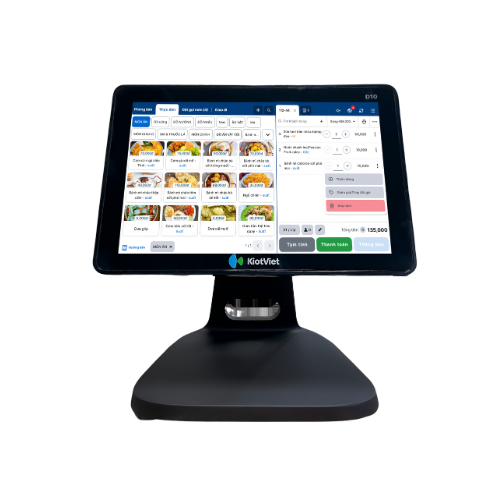
\includegraphics[width=15cm]{Images/kiosViet.png}
%     \caption{Máy POS KiotViet D10. Nguồn: \href{https://www.kiotviet.vn/top-4-may-tinh-tien-cho-quan-an-quan-cafe-tot-nhat-hien-nay/}{kiotviet.vn}}
% \end{figure}

% Mặc dù công nghệ đã mang lại những bước tiến vượt bậc, ngành nhà hàng vẫn phải đối mặt với một số thách thức lớn. Lạm phát và chi phí thực phẩm tăng cao đang tạo ra áp lực nặng nề, khiến hơn 30.000 cơ sở nhà hàng phải đóng cửa trong nửa đầu năm 2024 \cite{USDA}. Thêm vào đó, thiếu hụt lao động, đặc biệt là nhân viên có tay nghề cao, và các vấn đề liên quan đến chuỗi cung ứng cũng khiến các nhà hàng gặp khó khăn trong việc duy trì hoạt động hiệu quả. Gián đoạn toàn cầu ảnh hưởng đến nguồn cung nguyên liệu, làm gia tăng chi phí và giảm tính linh hoạt trong quản lý. Tuy nhiên, những thách thức này cũng tạo cơ hội lớn để đổi mới và cải tiến. Bên cạnh đó, sự phát triển mạnh mẽ của các nền tảng giao đồ ăn trực tuyến và thương mại điện tử đã mở ra những kênh doanh thu mới, giúp ngành nhà hàng không chỉ duy trì mà còn gia tăng sự phát triển. \\

% Nhờ vào sự cải tiến liên tục trong công nghệ, ngành nhà hàng tại Việt Nam đã và đang chứng kiến những bước tiến vượt bậc trong việc nâng cao chất lượng dịch vụ và cải thiện trải nghiệm khách hàng. Các giải pháp như hệ thống POS hiện đại, ứng dụng di động để đặt món và theo dõi giao hàng, cũng như sự tích hợp trí tuệ nhân tạo đã giúp các nhà hàng hoạt động hiệu quả hơn và đáp ứng nhu cầu ngày càng cao của khách hàng. Sự gia tăng dịch vụ giao đồ ăn trực tuyến càng làm cho việc ăn uống trở nên tiện lợi hơn, đặc biệt là ở các khu vực đô thị, khi mà khách hàng có thể dễ dàng đặt món và thanh toán qua các ví điện tử. Các nhà hàng không chỉ đơn giản là cung cấp thực phẩm, mà còn đang mang lại trải nghiệm mua sắm thuận tiện, nhanh chóng và an toàn cho khách hàng. \\

% Ngành công nghiệp nhà hàng tại Việt Nam hiện nay đang ở một ngã rẽ quan trọng, khi công nghệ đóng vai trò trung tâm trong sự phát triển của ngành. Mặc dù vẫn còn những thách thức đáng kể, việc áp dụng công nghệ chiến lược mang lại cơ hội lớn cho các doanh nghiệp nhà hàng. Tích hợp các hệ thống POS tiên tiến, ứng dụng di động giúp tối ưu hóa các hoạt động, tạo ra những cải tiến đáng kể trong trải nghiệm khách hàng. Trong khi thị trường tiếp tục phát triển, việc ứng dụng công nghệ sẽ là yếu tố then chốt giúp các nhà hàng duy trì sự cạnh tranh và đáp ứng nhu cầu thay đổi của khách hàng trong kỷ nguyên số.








\subsection{Giới thiệu đề tài}

Tính đến năm 2023, ngành dịch vụ thực phẩm (bao gồm khách sạn, nhà hàng và dịch vụ thể chế) đã đạt tổng giá trị 26,9 tỷ USD, với mức tăng trưởng 14,7\%. Mặc dù phải đối mặt với nhiều thách thức như lạm phát, chi phí vận hành tăng cao và sự cạnh tranh khốc liệt, ngành này đã phục hồi mạnh mẽ và gần như đạt doanh thu tương đương với thời kỳ trước đại dịch. Trong nửa đầu năm 2024, doanh thu từ dịch vụ lưu trú, thực phẩm và đồ uống đạt 24,1 tỷ USD, tăng 12,5\% so với cùng kỳ năm trước \cite{USDA}. 

\begin{figure}[H]
    \centering
    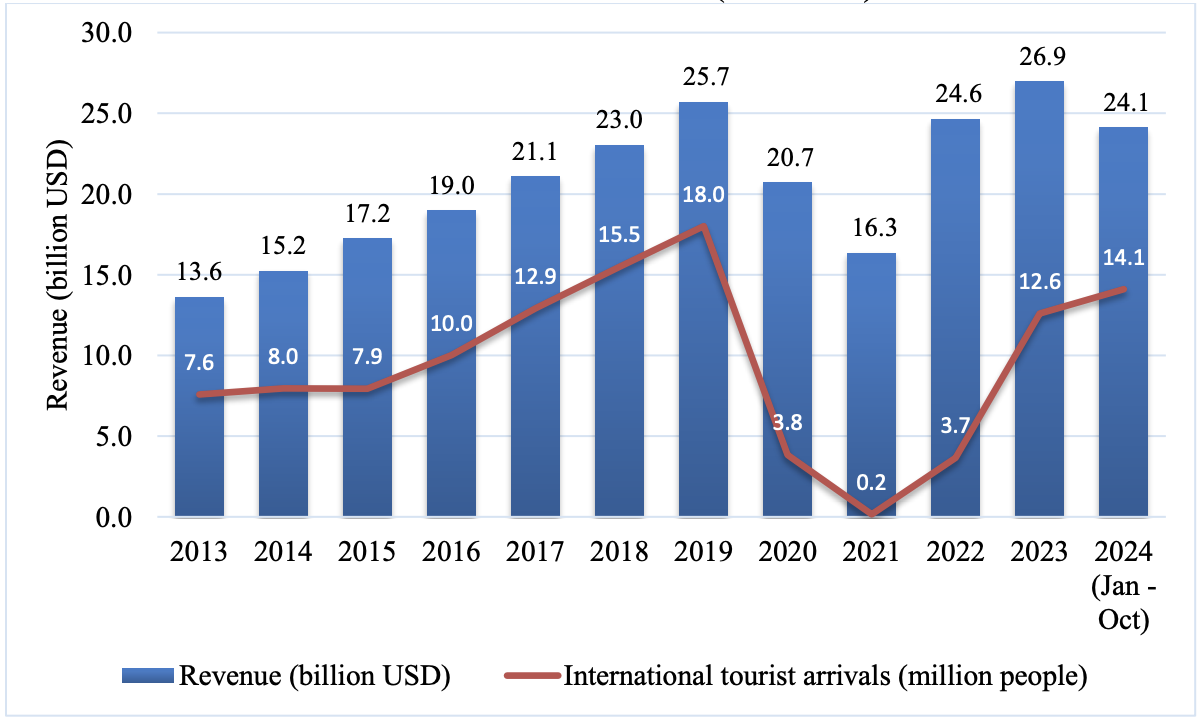
\includegraphics[width=15cm]{Images/resindus.png}
    \caption{Doanh thu từ Dịch vụ Lưu trú, Ăn uống và Số lượng Du khách Quốc tế từ năm 2013 đến năm 2024. Nguồn: Post calculations; Vietnam’s General Statistics Office.}
    \label{fig:enter-label}
\end{figure}

Trong bối cảnh công nghệ số ngày càng phát triển mạnh mẽ, việc áp dụng các giải pháp công nghệ vào quản lý và vận hành doanh nghiệp không chỉ là xu hướng mà còn là yếu tố quan trọng giúp nâng cao hiệu quả hoạt động và cải thiện trải nghiệm khách hàng. Đặc biệt, đối với ngành dịch vụ ăn uống, đặc biệt là các nhà hàng, việc quản lý quy trình đặt món và phục vụ khách hàng có thể gặp nhiều khó khăn và thách thức do tính chất phức tạp của công việc, cũng như yêu cầu phải đáp ứng nhu cầu đa dạng của khách hàng.

Phương pháp quản lý truyền thống, dựa chủ yếu vào ghi chép thủ công và giao tiếp trực tiếp, đã bộc lộ nhiều hạn chế, chẳng hạn như dễ mắc sai sót, khó theo dõi lịch sử đặt món và tốn thời gian trong quá trình vận hành. Những vấn đề này không chỉ làm giảm hiệu quả công việc mà còn ảnh hưởng xấu đến trải nghiệm của khách hàng, đặc biệt là trong môi trường cạnh tranh ngày càng gay gắt trong ngành.

Sự tích hợp công nghệ đã và đang đóng vai trò then chốt trong việc thay đổi sâu sắc ngành công nghiệp nhà hàng, mang đến những bước đột phá trong hoạt động và trải nghiệm khách hàng. Các công nghệ hiện đại không chỉ giúp cải thiện hiệu quả vận hành mà còn tối ưu hóa các quy trình và nâng cao chất lượng dịch vụ. Dưới đây là những công nghệ nổi bật đang làm thay đổi ngành nhà hàng:
\begin{enumerate}
    \item \textbf{Hệ Thống POS (Điểm Bán Hàng)}: Các hệ thống POS hiện nay không chỉ đơn giản là máy tính tiền mà đã phát triển thành những giải pháp toàn diện, hỗ trợ các nhà hàng trong việc quản lý đơn hàng, theo dõi tồn kho và phân tích xu hướng bán hàng. Với sự hỗ trợ của POS, các chủ nhà hàng có thể đưa ra các quyết định sáng suốt, tối ưu hóa các hoạt động quản lý và tăng cường lợi thế cạnh tranh, giúp duy trì sự phát triển bền vững trong một ngành công nghiệp luôn thay đổi.
    \item \textbf{Đặt Món Trực Tuyến (Online)}: Thói quen tiêu dùng tại Việt Nam đang thay đổi mạnh mẽ với sự ưa chuộng các giao dịch số và thanh toán trực tuyến. Dịch vụ giao đồ ăn trực tuyến đã trở thành một phần không thể thiếu trong thói quen của nhiều người, đặc biệt là ở các thành phố lớn. Theo thống kê, trong năm 2023, chi tiêu của người tiêu dùng Việt Nam cho dịch vụ giao đồ ăn tăng 30\%, đạt mức 1,4 tỷ USD, mức tăng trưởng cao nhất trong khu vực Đông Nam Á \cite{USDA}. Các nhà hàng đang tận dụng mạnh mẽ kênh giao đồ ăn trực tuyến để thúc đẩy doanh thu và thu hút khách hàng mới. Ví dụ, KFC đã mở thêm các cửa hàng ảo trên các nền tảng thương mại điện tử như Shopee Food và Grab Food, đồng thời sử dụng TikTok để livestream và cung cấp các ưu đãi hấp dẫn, gia tăng sự tương tác với khách hàng và đảm bảo giao hàng nhanh chóng trong vòng một giờ.
\end{enumerate}

\begin{figure}[H]
    \centering
    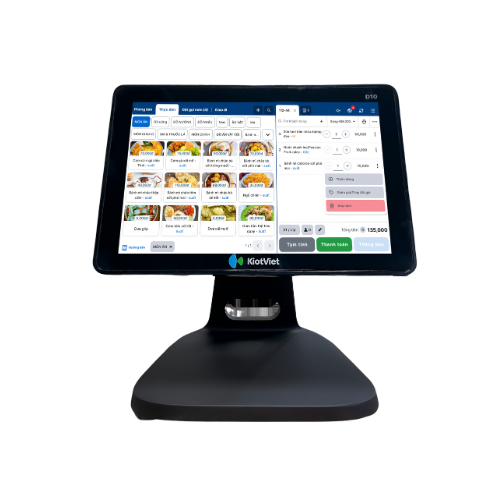
\includegraphics[width=10cm]{Images/kiosViet.png}
    \caption{Máy POS KiotViet D10. Nguồn: \href{https://www.kiotviet.vn/top-4-may-tinh-tien-cho-quan-an-quan-cafe-tot-nhat-hien-nay/}{kiotviet.vn}}
\end{figure}

Mặc dù công nghệ đã mang lại những bước tiến vượt bậc, ngành nhà hàng vẫn phải đối mặt với một số thách thức lớn. Lạm phát và chi phí thực phẩm tăng cao đang tạo ra áp lực nặng nề, khiến hơn 30.000 cơ sở nhà hàng phải đóng cửa trong nửa đầu năm 2024 \cite{USDA}. Thêm vào đó, thiếu hụt lao động, đặc biệt là nhân viên có tay nghề cao, và các vấn đề liên quan đến chuỗi cung ứng cũng khiến các nhà hàng gặp khó khăn trong việc duy trì hoạt động hiệu quả. Gián đoạn toàn cầu ảnh hưởng đến nguồn cung nguyên liệu, làm gia tăng chi phí và giảm tính linh hoạt trong quản lý. Tuy nhiên, những thách thức này cũng tạo cơ hội lớn để đổi mới và cải tiến. Bên cạnh đó, sự phát triển mạnh mẽ của các nền tảng giao đồ ăn trực tuyến và thương mại điện tử đã mở ra những kênh doanh thu mới, giúp ngành nhà hàng không chỉ duy trì mà còn gia tăng sự phát triển.

Dự án này được triển khai nhằm giải quyết những vấn đề đó thông qua việc xây dựng một hệ thống quản lý đặt món hiện đại. Hệ thống này không chỉ tự động hóa các quy trình từ việc đặt món, quản lý đơn hàng đến thanh toán, mà còn giúp nhà hàng dễ dàng mở rộng các tính năng như tối ưu hóa lịch làm việc của nhân viên và phân tích doanh thu.

Việc triển khai hệ thống quản lý đặt món hiện đại sẽ mang lại nhiều lợi ích cho cả khách hàng và nhà hàng. Khách hàng có thể dễ dàng tiếp cận thực đơn, đặt món nhanh chóng và thanh toán tiện lợi. Còn đối với nhà hàng, việc này giúp nâng cao hiệu quả vận hành, giảm thiểu chi phí và tối ưu hóa nguồn lực. Đây không chỉ là một bước tiến quan trọng trong việc cải thiện quy trình kinh doanh mà còn là nền tảng giúp các nhà hàng sẵn sàng hội nhập và phát triển bền vững trong kỷ nguyên số.

Nhờ vào sự cải tiến liên tục trong công nghệ, ngành nhà hàng tại Việt Nam đã và đang chứng kiến những bước tiến vượt bậc trong việc nâng cao chất lượng dịch vụ và cải thiện trải nghiệm khách hàng. Các giải pháp như hệ thống POS hiện đại, ứng dụng di động để đặt món và theo dõi giao hàng đã giúp các nhà hàng hoạt động hiệu quả hơn và đáp ứng nhu cầu ngày càng cao của khách hàng. Sự gia tăng dịch vụ giao đồ ăn trực tuyến càng làm cho việc ăn uống trở nên tiện lợi hơn, đặc biệt là ở các khu vực đô thị, khi mà khách hàng có thể dễ dàng đặt món và thanh toán qua các ví điện tử. Các nhà hàng không chỉ đơn giản là cung cấp thực phẩm, mà còn đang mang lại trải nghiệm mua sắm thuận tiện, nhanh chóng và an toàn cho khách hàng.

Ngành công nghiệp nhà hàng tại Việt Nam hiện nay đang ở một ngã rẽ quan trọng, khi công nghệ đóng vai trò trung tâm trong sự phát triển của ngành. Mặc dù vẫn còn những thách thức đáng kể, việc áp dụng công nghệ chiến lược mang lại cơ hội lớn cho các doanh nghiệp nhà hàng. Tích hợp các hệ thống POS tiên tiến, ứng dụng di động giúp tối ưu hóa các hoạt động, tạo ra những cải tiến đáng kể trong trải nghiệm khách hàng. Trong khi thị trường tiếp tục phát triển, việc ứng dụng công nghệ sẽ là yếu tố then chốt giúp các nhà hàng duy trì sự cạnh tranh và đáp ứng nhu cầu thay đổi của khách hàng trong kỷ nguyên số.